\section{仿真方案与原生波形分析}
\subsection{分层验证和覆盖范围}
验证采用软件参考、RTL 模块、链路集成和板卡验收四个层次。2026 年 10 月 9 日完成 59 项 Python 测试和表\ref{tab:sim}的 7 项 RTL 回归，并对 6 个板卡控制场景及 3 个摄像头场景的 JPEG 执行逐字节金样比较。同步 USB 集成仿真验证了 18 帧。

\begin{table}[H]\centering\caption{RTL 回归测试及主要覆盖项}\label{tab:sim}
\small\begin{tabularx}{\linewidth}{@{}p{61mm}Y@{}}\toprule
测试平台 & 覆盖内容\\\midrule
\nolinkurl{tb_camera_board_controls} & 去抖、长按单次触发、停止优先、原子提交及解析超时\\
\nolinkurl{tb_mjpeg_board_controls} & 画质表切换、帧生命周期、控制与编码协同\\
\nolinkurl{tb_mjpeg_real_camera} & DVP、像素 CDC、编码、MBLK、短行 abort 及恢复\\
\nolinkurl{tb_mjpeg_payload_coalescer} & 载荷归并、有效字节数、包结束\\
\nolinkurl{tb_mjpeg_block_transport} & 分块、描述符和状态复用\\
\nolinkurl{tb_board_test_async_fifo} & 异步读写、满队列、回绕、停钟和数据保持\\
\nolinkurl{tb_davinci_mjpeg_sync_test} & 同步 FT245 总线与完整 JPEG 输出集成\\\bottomrule
\end{tabularx}\end{table}

\subsection{本次波形导出的范围}
2026 年 10 月 25 日补跑板卡控制和摄像头链路两项测试，启用调试可见性并导出 VCD/WDB，随后使用 Vivado 2020.1 原生窗口截图。WDB 保存波形活动，WCFG 保存信号、时间范围和列宽等显示配置\cite{ug900}。正文裁取原生波形区域以保证字号可读，完整窗口 PNG 和数据库仍保留在工程附件中。

摄像头测试使用 $48\times16$ 的 YUYV 激励，核心时钟周期 10 ns、PCLK 周期 40 ns，并随机拉低输出 ready。它检验采集、CDC、JPEG 与封包的集成关系，不直接复现生产链路 RAW8 颜色重建、1080p 尺寸及所有模拟器件行为。后者需要结合对应软件参考和实板结果判断。

软件测试覆盖当前图像参考、主机协议和控制行为，独立 JPEG 金样提供字节级确定性验证；实拍图像不能与固定金样逐字节比较，应检查格式、连续性、错误状态、尺寸与完整解码。分层判定有助于区分算法错误、封包错误和器件连接问题。
\evid{mjpeg/docs/精简验证.json；waveforms_20261025/waveform_summary.json}
\clearpage

\subsection{摄像头完整帧、故障与恢复}
\begin{figure}[H]\centering
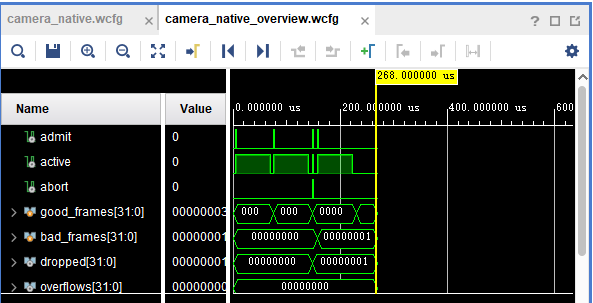
\includegraphics[width=.86\linewidth]{native_camera_crop.png}
\caption{Vivado 原生摄像头链路波形区域。最终成功 3、失败 1、丢弃 1、溢出 0；总线值沿用原生窗口基数。}\label{fig:simcamera}
\end{figure}
图\ref{fig:simcamera}中，\texttt{admit} 允许新帧进入，\texttt{active} 覆盖接收区间。测试在第三次尝试中仅发送 13 个像素构造短行，触发一次 \texttt{abort}，失败与丢弃计数各增一次；随后完整帧再次成功，最终 \texttt{good\_frames=3}。该失败是预期测试事件，不代表正常输入下的随机丢帧。

\begin{figure}[H]\centering
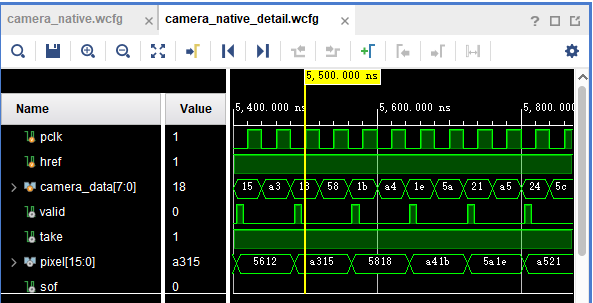
\includegraphics[width=.86\linewidth]{native_pixels_crop.png}
\caption{Vivado 原生像素握手细节，约 5.4～5.8 $\mu$s；光标为 5500 ns。}\label{fig:simpixel}
\end{figure}
图\ref{fig:simpixel}显示 PCLK、HREF 和 8 位输入字节，捕获后形成 16 位 YUV422 像素。\texttt{valid} 与 \texttt{take} 共同决定接受时刻；总线上的保持区间不代表重复接受。SOF/EOL/EOF 仅在像素 valid 有效时具有语义，分析时须同时观察握手。
\evid{camera.wdb；vivado_camera_overview.png；vivado_pixel_handshake.png}
\clearpage

\subsection{板卡控制波形和测试激励}
\begin{figure}[H]\centering
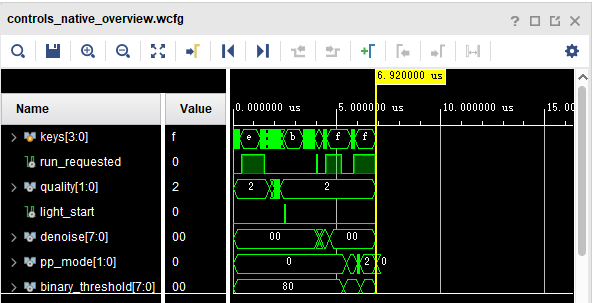
\includegraphics[width=.93\linewidth]{native_controls_crop.png}
\caption{Vivado 原生控制波形：按键、运行请求、画质、降噪强度与模式设置。}\label{fig:simcontrols}
\end{figure}
图\ref{fig:simcontrols}中按键低有效。测试构造抖动、长按、单次按键和 USB 字节，检查运行请求不会由接点抖动反复翻转。\texttt{quality} 的内部编码 0/1/2 对应 Q60/Q75/Q85。降噪和模式设置在完整命令结束时改变，非法模式和畸形载荷不能提交或泄漏为启停、补光。

代码\ref{lst:test}列出摄像头仿真的主要激励：前两帧正常，第三次发送短行，之后发送含帧中 STOP 的完整帧并等待输出。
\lstinputlisting[language=Verilog,firstnumber=86,caption={摄像头测试中的故障注入和恢复检查},label={lst:test}]{code/sim_fault_recovery.sv}
\src{mjpeg/tb/tb_mjpeg_real_camera.sv:86--92}

\subsection{通过判定和复核}
测试平台通过断言和最终 PASS 标记检查结果。工具正常退出不足以替代断言检查，脚本还检索 \texttt{Fatal:} 和目标标记。摄像头场景必须同时满足 3 帧成功、1 次失败、1 次 abort、3 帧接收、1 次丢弃和 0 次溢出。完整 VCD 可进一步放大脉冲，WDB/WCFG 可恢复原生显示。
\evid{BUTTON_DEBOUNCE_PASS.txt；REAL_CAMERA_SIM_PASS.txt；simulation.log}
\clearpage
